\chapter{Security architecture for AI coding agents}

\section{Engineering principles}

The main trust boundary is between untrusted context and authorized effects. Repository files, issues, tool results, generated patches and memory can all carry adversarial content. Threats include injection, credential theft, malicious command execution, dependency compromise and unauthorized modification. A defense-in-depth design combines identity, isolation, egress control, policy, review and evidence.\src{W1,O5,A6,A8,M1}

\section{Implementation approach}

Model assets, actors, entry points, trust boundaries and data flows. Deny production credentials and direct deployment access. Restrict network destinations; validate tool inputs at the server; keep task workspaces ephemeral. Store approval decisions externally and bind them to a specific commit. Scan diffs and dependencies, quarantine suspicious artifacts and retain audit records with redaction.

\section{Verification and limitations}

Exercise adversarial fixtures and deny actions outside scope. Residual risks include unknown vulnerabilities, compromised approved dependencies, correlated verifier defects and data inferred from allowed outputs. The threat matrix in the package identifies owners and recovery steps.

Figure~\ref{fig:d19} illustrates the conceptual flow from Untrusted input to Scoped resources. The edges describe the proposed integration or control relationship, not undocumented internal calls.

\begin{figure}[htbp]\centering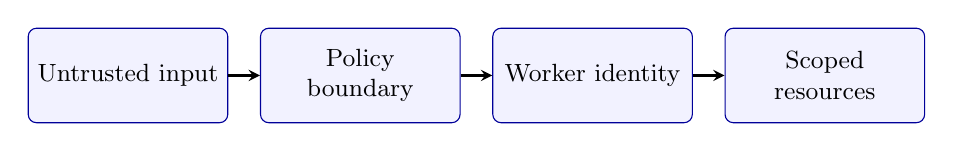
\begin{tikzpicture}[nodebox/.style={draw=blue!60!black,fill=blue!5,rounded corners=3pt,minimum height=12mm,text width=23mm,align=center,font=\small},>=stealth]
\node[nodebox] (n0) at (0.00,0.00) {Untrusted input};
\node[nodebox] (n1) at (2.95,0.00) {Policy boundary};
\node[nodebox] (n2) at (5.90,0.00) {Worker identity};
\node[nodebox] (n3) at (8.85,0.00) {Scoped resources};
\draw[->,thick] (n0.east) -- (n1.west);
\draw[->,thick] (n1.east) -- (n2.west);
\draw[->,thick] (n2.east) -- (n3.west);
\end{tikzpicture}
\caption{Security trust boundaries (conceptual view).}\label{fig:d19}\end{figure}

Figure~\ref{fig:d20} illustrates the conceptual flow from Tool proposal to Audit record. The edges describe the proposed integration or control relationship, not undocumented internal calls.

\begin{figure}[htbp]\centering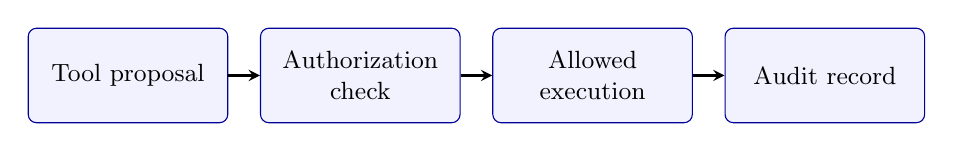
\begin{tikzpicture}[nodebox/.style={draw=blue!60!black,fill=blue!5,rounded corners=3pt,minimum height=12mm,text width=23mm,align=center,font=\small},>=stealth]
\node[nodebox] (n0) at (0.00,0.00) {Tool proposal};
\node[nodebox] (n1) at (2.95,0.00) {Authorization check};
\node[nodebox] (n2) at (5.90,0.00) {Allowed execution};
\node[nodebox] (n3) at (8.85,0.00) {Audit record};
\draw[->,thick] (n0.east) -- (n1.west);
\draw[->,thick] (n1.east) -- (n2.west);
\draw[->,thick] (n2.east) -- (n3.west);
\end{tikzpicture}
\caption{Permission enforcement (conceptual view).}\label{fig:d20}\end{figure}

\section{Chapter conclusion}

Apply the stated verification criteria before expanding the scope of this workflow. Record deviations, evidence and unresolved risks in the task record.
